\chapter{Fonction de transfert}
\section{Modèle du quadripôles}
\begin{figure}[ht]
  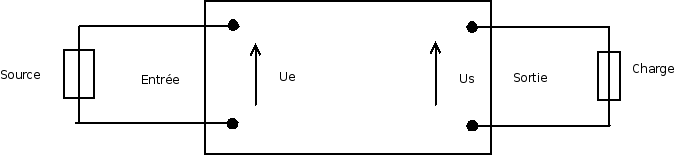
\includegraphics[width=12cm]{quadripole.png}
  \caption{Modèle du quadripôle}
\end{figure}
Si la source est une source de tension, on étudiera le cas où la source délivre un signal sinusoïdale ou échelon\\
Dans le cas sinusoïdale, on défini deux sous circuits : \\
\begin{figure}[ht]
  \centering
  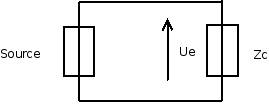
\includegraphics[width=5cm]{Physique/source.png}
  \caption{La source}
\end{figure}
\begin{figure}[ht]
  \centering
  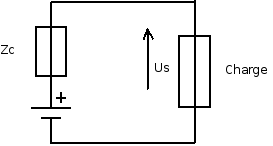
\includegraphics[width=6cm]{charge.png}
  \caption{La charge}
\end{figure}
\section{Fonction de transfert complexe}
\begin{de}
Dans le cas d'une sources fournissant un signal sinusoïdale, on défini une fonction de transfert par : 
$$H (j\omega) = \dfrac{\underline{X}_s}{\underline{X}_e}$$
avec :
\begin{itemize}
 \item[$\rightarrow$] $\underline{X}_s$ : Grandeur de sortie (Tension ou intensité)
 \item[$\rightarrow$] $\underline{X}_e$ : Grandeur d'entrée (Tension ou intensité)
\end{itemize}
Ces fonction de transfert sont sans dimensions.
\end{de}
\subsection{Amplitude}
Soit $\omega$ une pulsation, définie en rad.$s^{-1}$.\\
On associe à $\omega$ une fonction de transfert $H(j\omega)$.\\
\begin{de}
On appelle amplitude de H le module de H. 
$$(\mbox{ A est l'amplitude de H }) \Leftrightarrow ( A = |H(j\omega)|)$$
\end{de}
\subsection{Gain en décibel}
\begin{de}
On défini le gain en décibel d'une fonction de transfert par : 
$$G_{dB} = 20.log(|H(j\omega)|)$$
On utilise une échelle logarithmique pour pouvoir couvrir un large spectre de fréquence.
\end{de}
\subsection{Bande passante}
\begin{de}
On défini une bande passant comme l'ensemble des fréquences $\left\lbrace f \right\rbrace $ vérifiant :
$$| H(j2\pi f) | \geq \dfrac{H_{max}}{2} $$
\end{de}
\subsection{Phase}
\begin{de}
La phase de la fonction de transfert H($j\omega$) est l'argument de celui-ci.
\end{de}
\section{Représentations}
\subsection{Diagramme de Bode}
On défini deux graphiques : 
\begin{itemize}
 \item[$\rightarrow$] Celui du Gain : log(f) en abscisse, $G_{dB}$ en ordonnée
 \item[$\rightarrow$] Celui de la phase : log(f) en abscisse, $\varphi$ en ordonnée
\end{itemize}
\subsection{Diagramme de Nykwest}
On défini, dans le plan complexe, un point M qui à pour module $|H(j\omega)|$ et pour angle par rapport à l'axe de réel, $\varphi$
\section{Lien entre régime transitoire et fonction de transfert}
\subsection{Précaution d'utilisation}
Pour pouvoir utiliser ce procéder qui permet d'obtenir l'équation temporelle d'après la fonction de transfert, il faut que, lors de l'obtention de la fonction de transfert, si il existe plusieurs dipôles identiques dans le circuit, on les ai considérés de façon différente (ex : Si il y a deux résistance de valeur R, on pose qu'une est de valeur R, l'autre de valeur R', même si R=R').\\
A partir de là, on peut passer en temporel, et une fois l'équation différentielle obtenu, on utilise le faite que R=R'.
\subsection{Principe}
Considérons un quadripole. Pour déterminer l'équation différentielle relative au régime transitoire, on peut utiliser la fonction de transfert.\\
On considère donc que le circuit fonctionne en régime sinusoïdale. Une fois la fonction de transfert établie, on remplace les $(j\omega)^n\underbar{X}^n$ par $\dfrac{d^nX}{dt^n}$, et on obtient l'équation différentielle qui régit le système en régime transitoire.
\section{Type de réponse}
\subsection{Réponse indicielle}
La réponse indicielle est la réponse du système à un échelon.
\subsection{Réponse impulsionelle}
La réponse impulsionelle est la réponse du système à un échelon de longueur $\tau$.
\begin{prop}
Dans ce cas, on obtient la propriété suivante, qui est une propriété des transformée de Fourier : 
$$BP.\tau = 1$$
\end{prop}
\section{Réponse d'un filtre à un signal périodique}
Soit e(t) la tension d'entrée du quadripole.\\
Si e(t) est de la forme : 
$$e(t) = E.cos(\omega t)$$
Alors s(t), la tension de sortie du quadripole est donnée par :
$$s(t) = |H(j\omega)|.E.cos(\omega t + Arg(H(j\omega))$$
\section{Caractère intégrateur ou dérivateur d'un filtre}
\subsection{Filtre intégrateur}
\begin{de}
On dit d'un filtre qu'il est intégrateur si :
$$s(t) = \dfrac{1}{a}.\int e(t)$$
ou
$$e(t) = a.\dfrac{ds(t)}{dt}$$
Ce qui signifie que la fonction de transfert du système est de la forme (Intégrateur idéal) : 
$$H(j\omega) = \dfrac{1}{ja\omega}$$
\end{de}
\subsection{Filtre dérivateur}
\begin{de}
On dit d'un filtre qu'il est dérivateur si :
$$s(t) = b.\dfrac{de(t)}{dt}$$
Ce qui signifie que la fonction de transfert du système est de la forme (Dérivateur idéal) : 
$$H(j\omega) = jb\omega$$
\end{de}

